\newpage

\section{Grúa}

La composición de la grúa la he realizado usando un cubo achatado, para la unión de ambas plataformas, y dos cubos también achatados para las propias plataformas.

\bigskip

% rescribir
Además, he puesto dos \textit{dummies} en el cubo que une ambas plataformas; es decir, en los extremos del brazo, con el objetivo de que funcione bien la restricción que explicaré a continuación. En cuanto a las plataformas, he movido sus pivotes para que se encuentren pegados a una de las caras, para que al usar la restricción no se solape con el brazo.

\bigskip

En cuanto a las restricciones, he usado un \textit{Position Constraint} en cada plataforma, con su \textit{Target} siendo su \textit{Dummy} respectivo. Esto hace que el brazo pueda girar junto a las plataformas, pero estas últimas siempre paralelas al suelo.

\bigskip

Cabe destacar que estas restricciones no tienen animaciones, al no tener otro objeto al que unirse.

% foto de los dummies, el pivote y general
\begin{figure}[H]
    \centering
    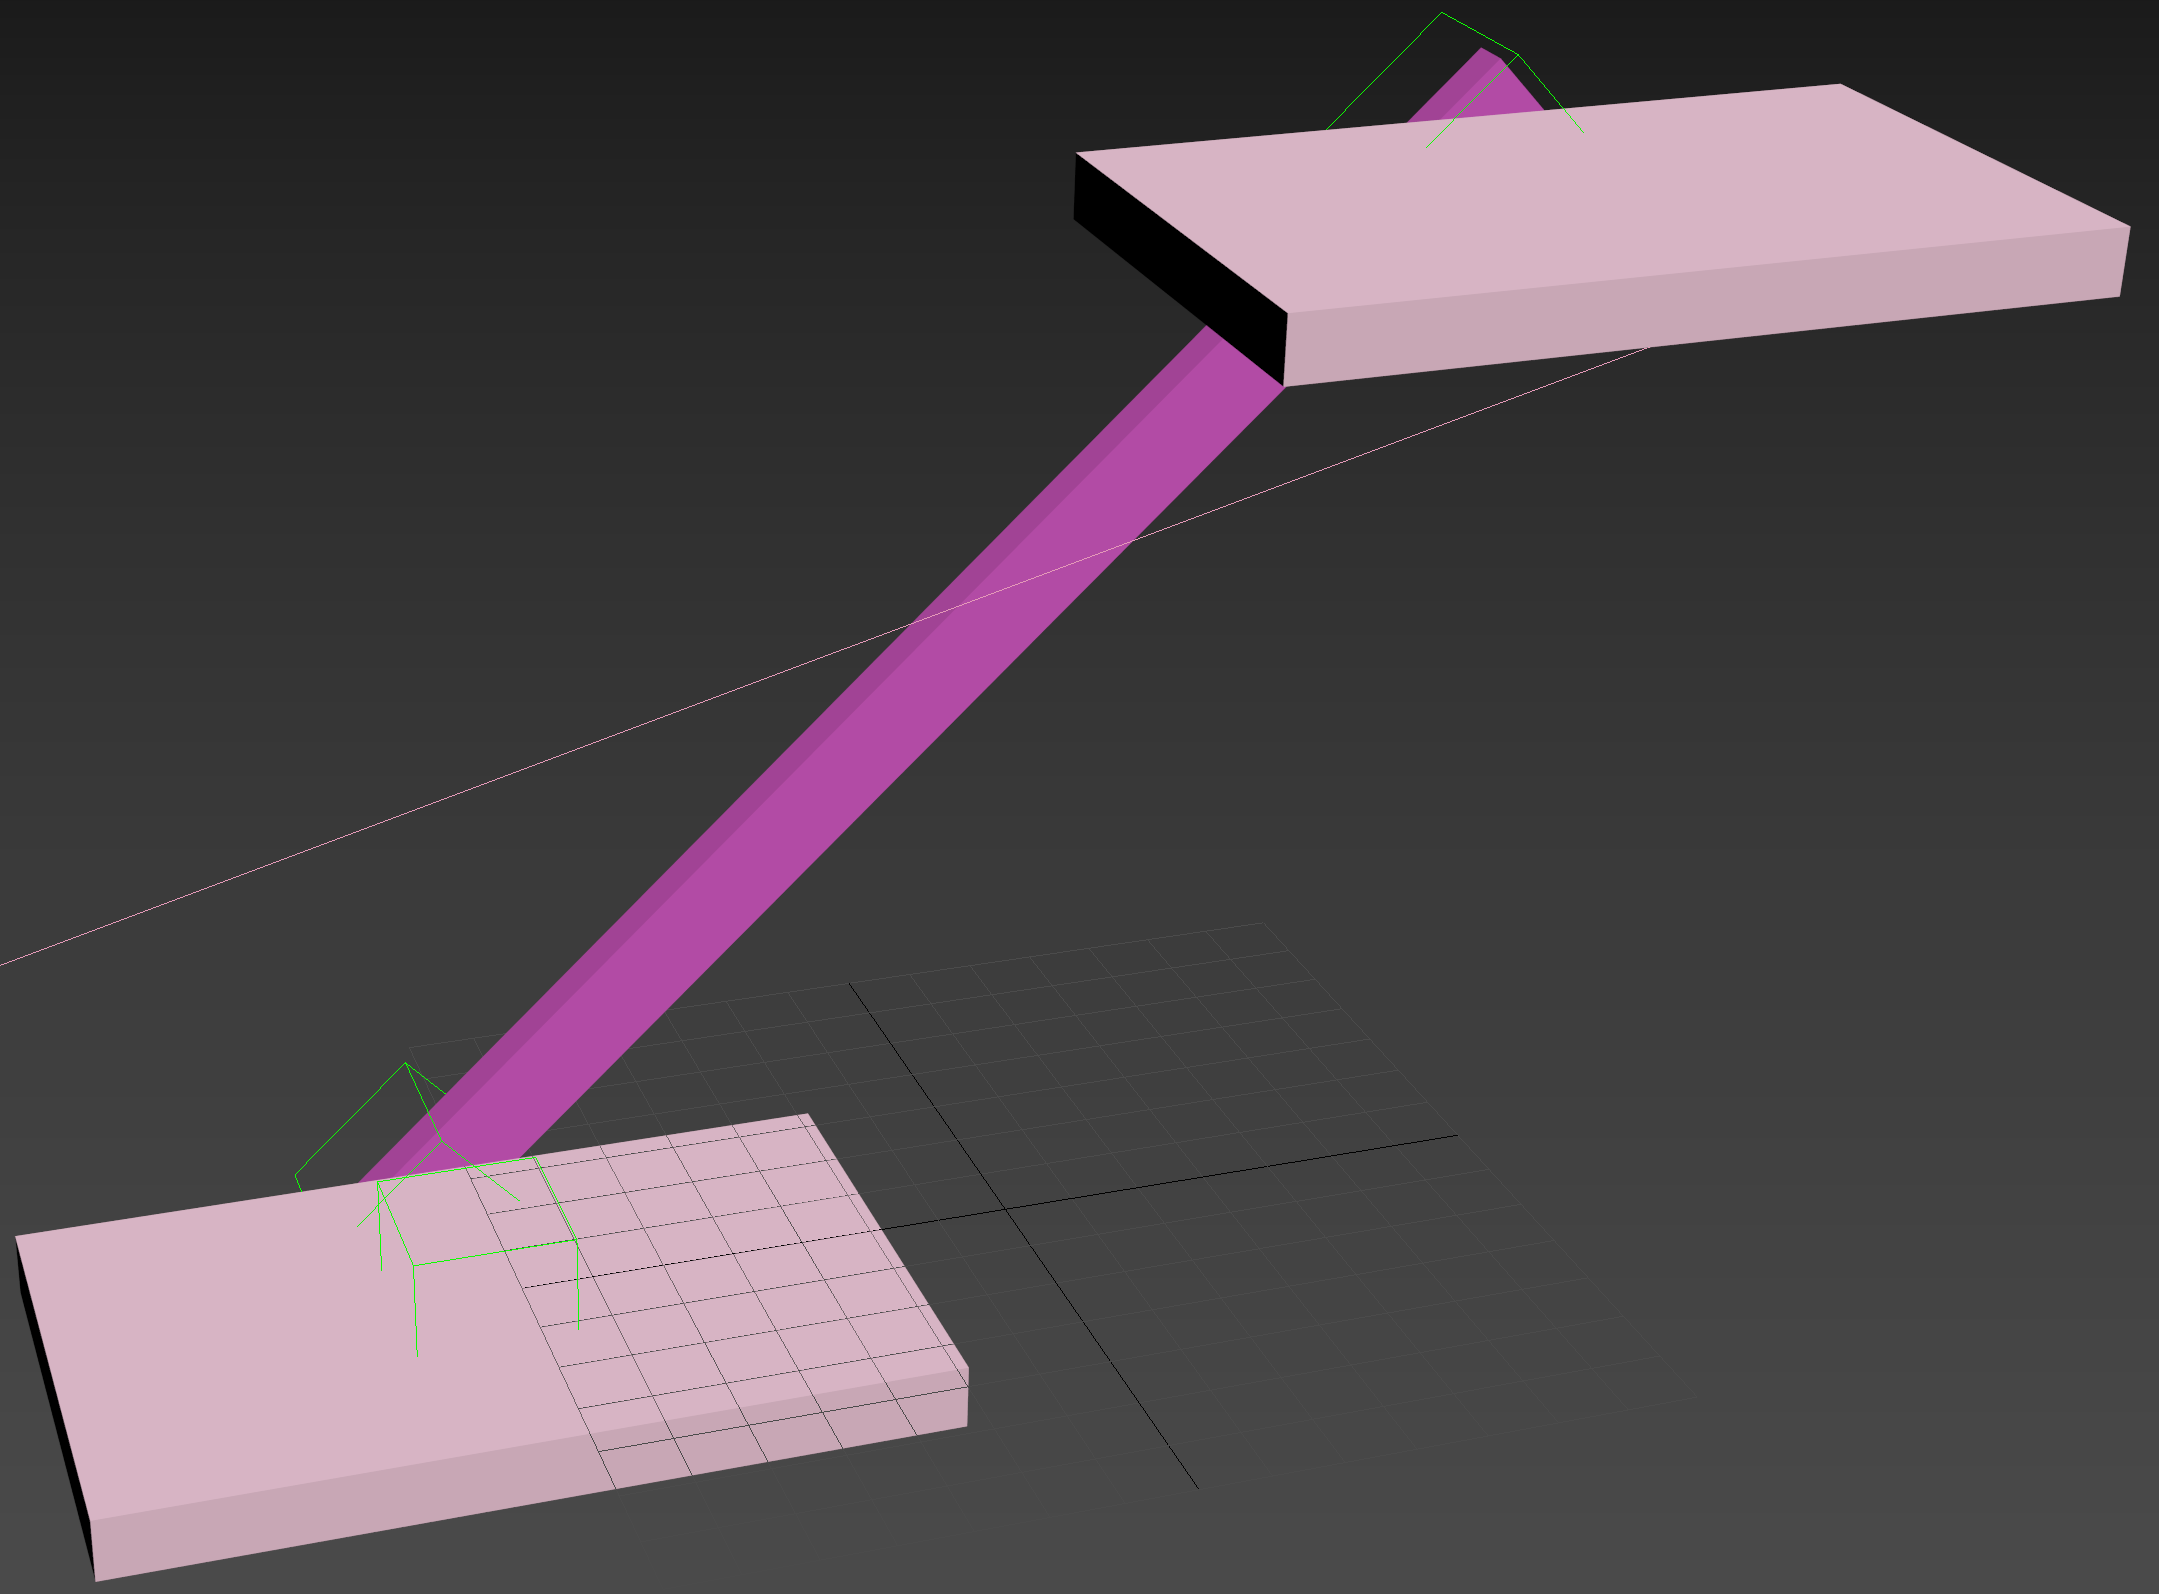
\includegraphics[width=0.6\textwidth]{imagenes/grua/grua.png}
    \caption{Forma final de la grúa.}
 \end{figure}

Los \textit{keyframes} de la grúa, más concretamente del brazo que gira, son:

\begin{itemize}
    \item \textbf{Instante 90: }Se encuentra en su posición inicial.
    \item \textbf{Instante 125: }El brazo ha girado y las plataformas han cambiado de posición, estando arriba la de abajo y viceversa.
\end{itemize}

\bigskip

La curva de animación para el brazo es:

% curva
\begin{figure}[H]
    \centering
    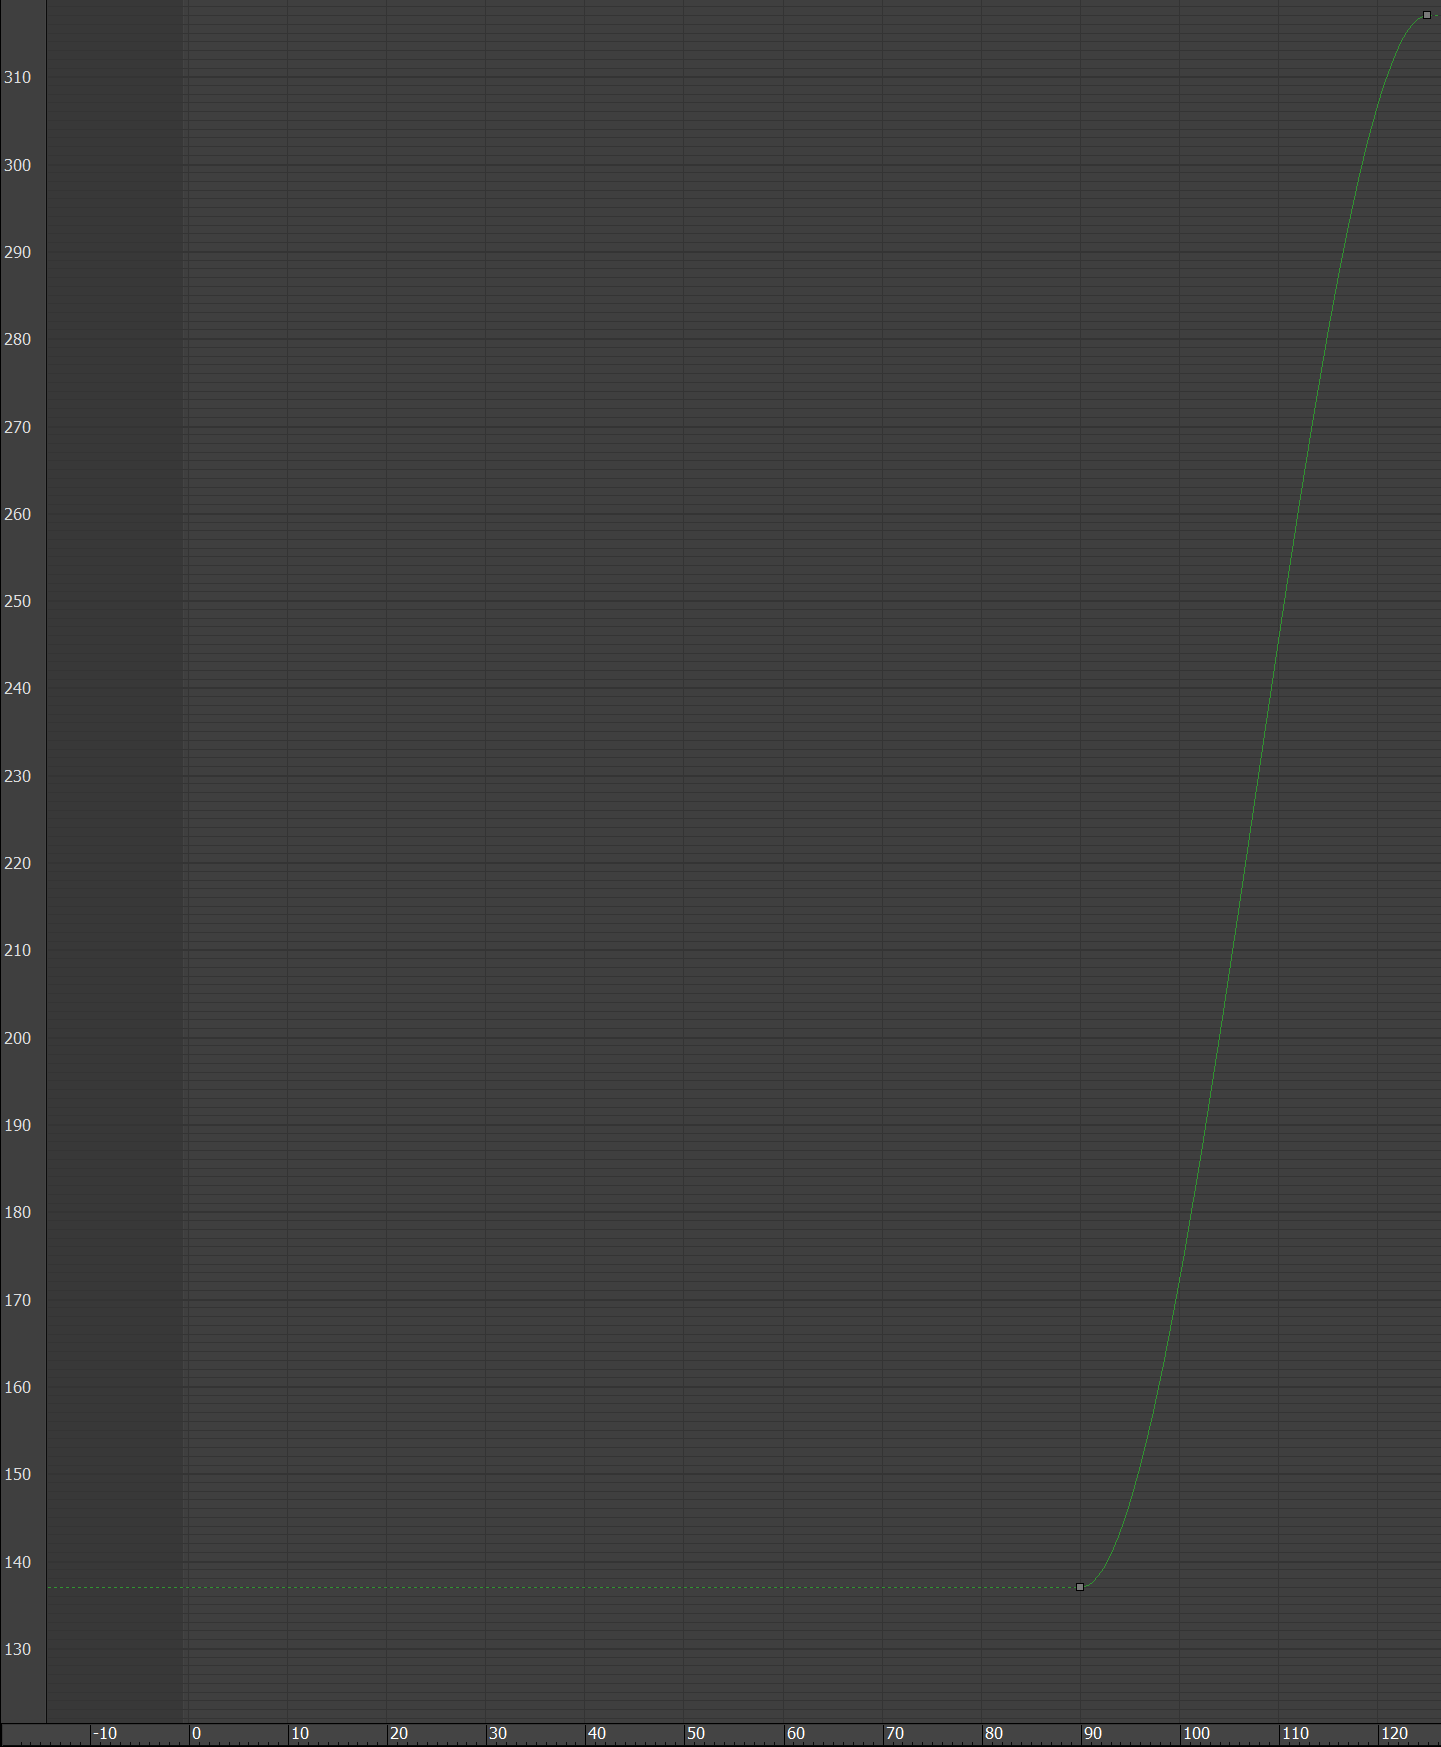
\includegraphics[width=0.5\textwidth]{imagenes/grua/rotY.png}
    \caption{Curva que representa la rotación en eje Y con respecto al tiempo.}
 \end{figure}

He vuelto a elegir una forma \textit{Slow-in/Slow-out} debido a que me parecía más realista que un motor tarde unas décimas de segundo en alcanzar la velocidad y también que requiera un tiempo en desacelerar.

\bigskip

Y los fotogramas más importantes después de haber hecho todo esto son:

% foto de los fotogramas mas imporantes.
\begin{figure}[H]
    \centering
\begin{subfigure}[t]{0.48\textwidth}
    \centering
    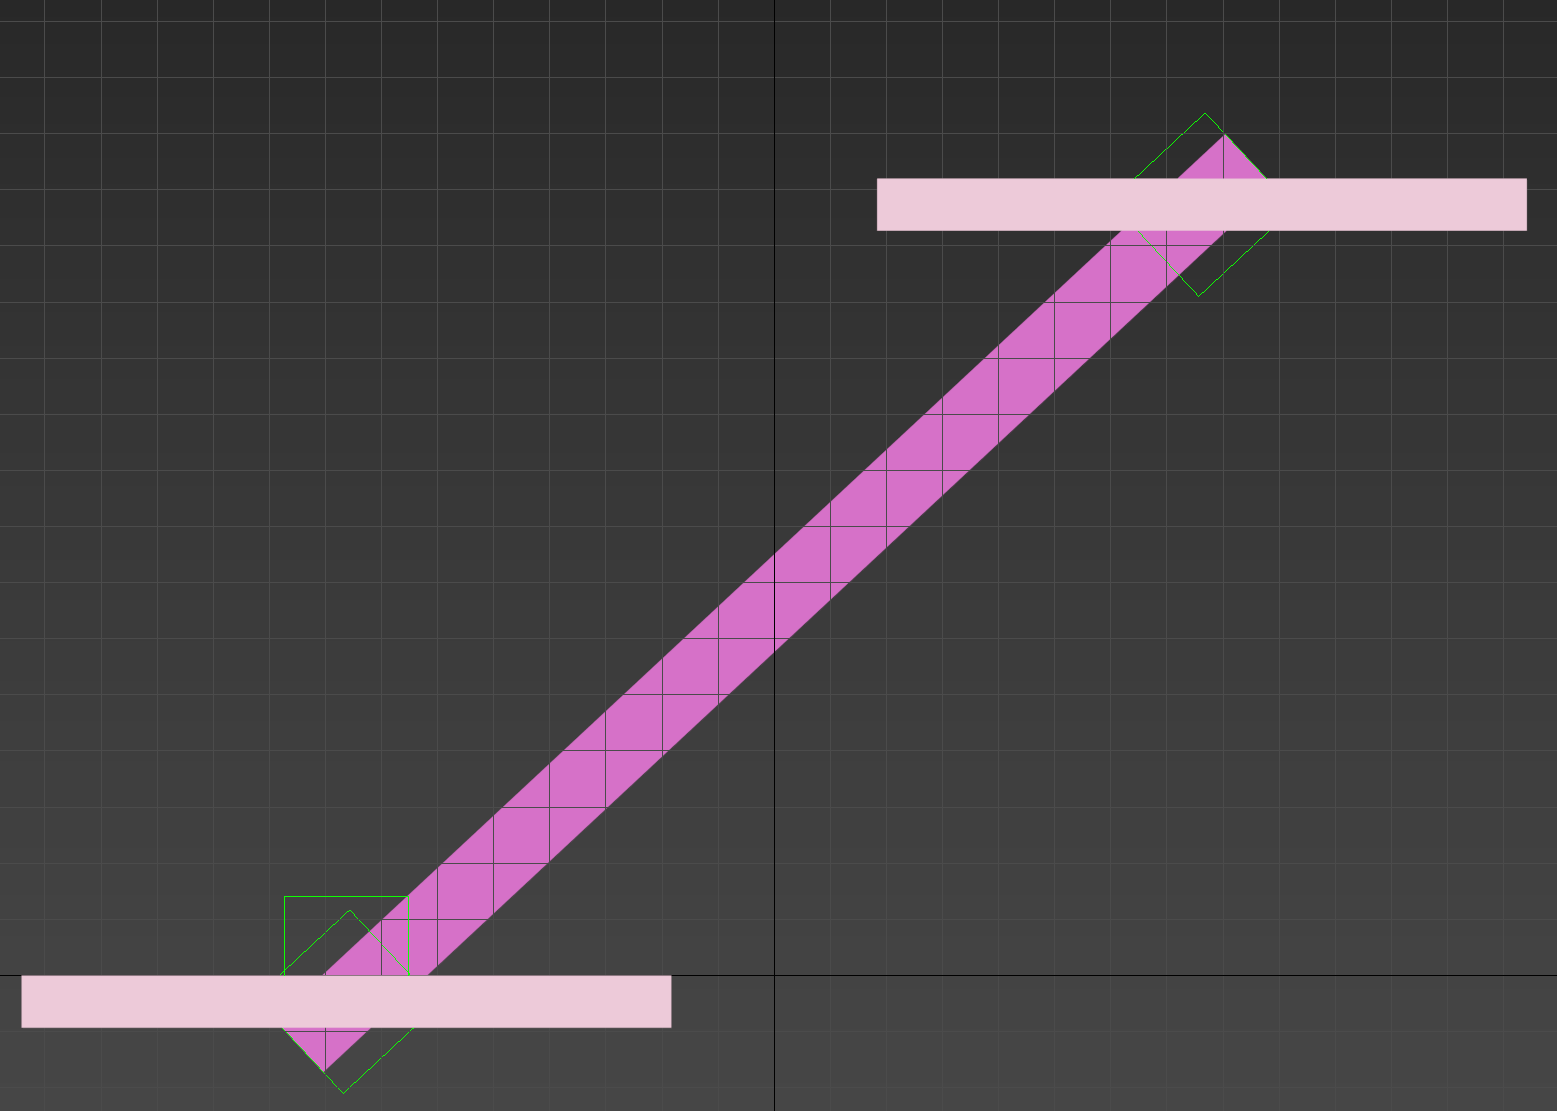
\includegraphics[width=\textwidth]{imagenes/grua/keyframes/90.png}
    \caption{Grúa en el instante 90 y anterior.}
 \end{subfigure}
\hfill
 \begin{subfigure}[t]{0.48\textwidth}
    \centering
    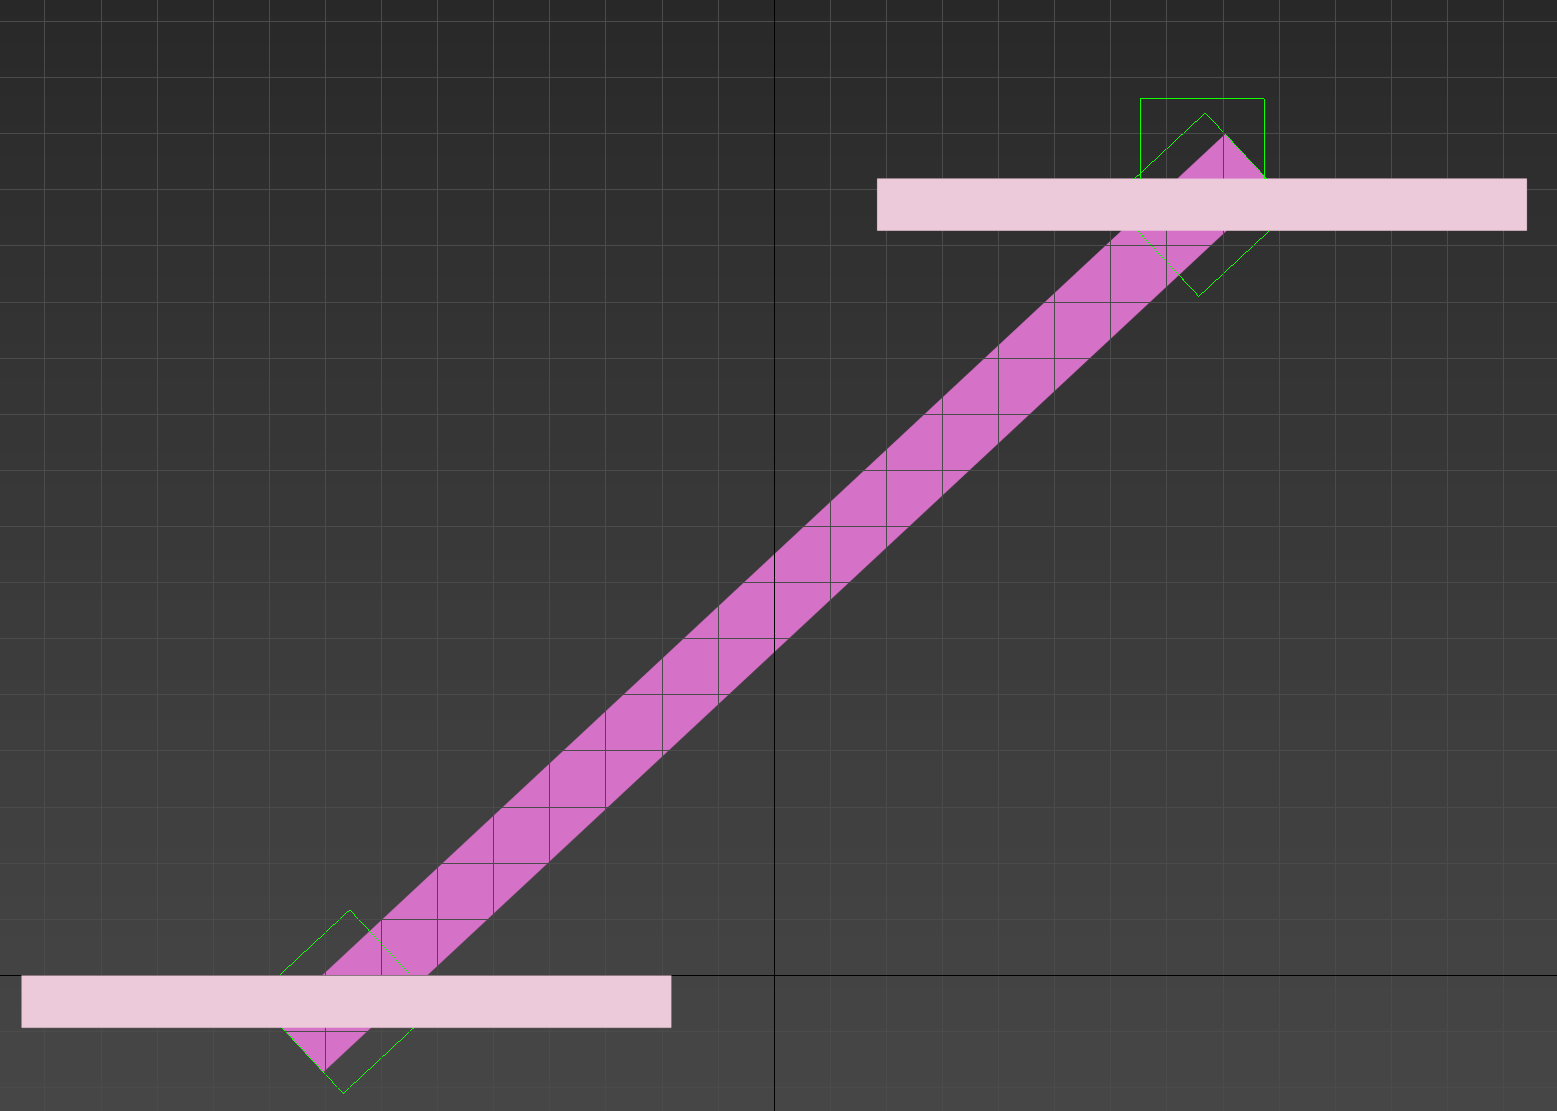
\includegraphics[width=\textwidth]{imagenes/grua/keyframes/125.png}
    \caption{Grúa en el instante 125 y siguientes.}
 \end{subfigure}
 \caption{\textit{Keyframes} de la grúa.}
\end{figure}